\documentclass{beamer}

\mode<presentation> {

% The Beamer class comes with a number of default slide themes
% which change the colors and layouts of slides. Below this is a list
% of all the themes, uncomment each in turn to see what they look like.

%\usetheme{default}
%\usetheme{AnnArbor}
\usetheme{Antibes}
%\usetheme{Bergen}
%\usetheme{Berkeley}
%\usetheme{Berlin}
%\usetheme{Boadilla}                
%\usetheme{CambridgeUS} %kkkkkkkkkkkk
%\usetheme{Copenhagen}
%\usetheme{Darmstadt}  % 22222222222222
%\usetheme{Dresden}
%\usetheme{Frankfurt}
%\usetheme{Goettingen} 
%\usetheme{Hannover} %llllllllllllll
%\usetheme{Ilmenau}
%\usetheme{JuanLesPins}
%\usetheme{Luebeck}
%\usetheme{Madrid} %3333333333333333333
%\usetheme{Malmoe}
%\usetheme{Marburg}
%\usetheme{Montpellier} %2222222
%\usetheme{PaloAlto}
%\usetheme{Pittsburgh}
%\usetheme{Rochester}
%\usetheme{Singapore}
%\usetheme{Szeged} % 0000000000000000
% \usetheme{Warsaw}

% As well as themes, the Beamer class has a number of color themes
% for any slide theme. Uncomment each of these in turn to see how it
% changes the colors of your current slide theme.

%\usecolortheme{albatross}
%\usecolortheme{beaver} % 0000000000
%\usecolortheme{beetle}
%\usecolortheme{crane}
\usecolortheme{dolphin} % 0000000
%\usecolortheme{dove}   %%%%%%%%%%
%\usecolortheme{fly}
%\usecolortheme{lily}
%\usecolortheme{orchid} %%%%%%%%%%%
%\usecolortheme{rose}
%\usecolortheme{seagull}
%\usecolortheme{seahorse}
%\usecolortheme{whale}
%\usecolortheme{wolverine}

%\setbeamertemplate{footline} % To remove the footer line in all slides uncomment this line
%\setbeamertemplate{footline}[page number] % To replace the footer line in all slides with a simple slide count uncomment this line

%\setbeamertemplate{navigation symbols}{} % To remove the navigation symbols from the bottom of all slides uncomment this line
}

\usepackage{graphicx} % Allows including images
\usepackage{booktabs} % Allows the use of \toprule, \midrule and \bottomrule in tables
\usepackage[brazil]{babel}
\usepackage[T1]{fontenc}	
\usepackage[utf8]{inputenc}	
\usepackage{verbatim}
\usepackage{xcolor,lipsum}
\usepackage{listings,showexpl}
\usepackage{amsmath}
\usepackage{fancybox}
\usepackage{verbatim}
\usepackage{graphicx}
\usepackage{url}
\usepackage{multicol}
\usepackage{parcolumns}
\usepackage{pxfonts}
\usepackage{transparent}
\usepackage[font=footnotesize,labelformat=empty,
            justification=raggedright,
%            singlelinecheck=false
  ]{caption}

\pdfcompresslevel=9
\pgfdeclareimage[width=2.5cm]{logo}{logo}
\logo{\transparent{0.2}\pgfuseimage{logo}}


%--------------------------------------------
%Definições para código com fundo listrado
\newcommand\realnumberstyle[1]{#1}
\makeatletter
\newcommand{\zebra}[3]{%
    {\realnumberstyle{#3}}%
    \begingroup
    \lst@basicstyle
    \ifodd\value{lstnumber}%
        \color{#1}\pgfsetfillopacity{0.9}%
    \else
        \color{#2}%
    \fi
        \rlap{\hspace*{\lst@numbersep}%
        \color@block{\linewidth}{\ht\strutbox}{\dp\strutbox}%
        }%
    \endgroup
}
\makeatother

\lstset{%
language=tex,           %linguagem
numbers=left,           %posição dos números
stepnumber=1,           %frequencia de aparição dos números
numbersep=5pt,
numberstyle=\zebra{black!10}{white!35},
basewidth={0.6em,0.45em},
linewidth=6cm,
fontadjust=true,
mathescape=true,
tabsize=4,
commentstyle=\color{blue},
literate={á}{{\'a}}1 {à}{{\`a}}1 {ã}{{\~a}}1 {é}{{\'e}}1 {É}{{\'E}}1 {ê}{{\^e}}1 {õ}{{\~o}}1 {í}{{\'i}}1 {ó}{{\'o}}1 {ú}{{\'u}}1 {ç}{{\c c}}1 {³}{{$^3$}}1 {¢}{{\$}}1 {Ω}{{$\Omega$}}1,
% use ¢ in local to $
breaklines=true,
showstringspaces=false,
stringstyle=\color{cyan},
basicstyle=\tiny\ttfamily}

\newcommand{\code}{\small\ttfamily}
% \defbeamertemplate{description item}{align left}{\insertdescriptionitem\hfill}
% \setbeamertemplate{description item}[align left]

\makeatletter
\newenvironment{CenteredBox}{% 
\begin{Sbox}}{% Save the content in a box
\end{Sbox}\centerline{\parbox{\wd\@Sbox}{\TheSbox}}}% And output it centered
\makeatother

 \usepackage{ragged2e}
%----------------------------------------------------------------------------------------
%	TITLE PAGE
%----------------------------------------------------------------------------------------

\title[Introdução ao \LaTeX]
{\textbf{\Large{Introdução ao \LaTeX}\\ uma abordagem prática}
}

\author[Lucas, Luiz, Pablo]{\textbf{Lucas Severo Alves\\
				Luiz F. G. Oliveira\\
				Pablo A. A. Urbizagástegui}} % Your name
\institute[FGA -- UnB] % Your institution as it will appear on the bottom of every slide, may be shorthand to save space
{
%Orientadora: Suélia de Siqueira Rodrigues Fleury Rosa\newline 

Faculdade UnB Gama -- FGA\\
Universidade de Brasília -- UnB\\
Laboratório de Engenharia Biomédica -- LAB\\

\medskip
\textit{lucassalves65@gmail.com\\ziuloliveira@gmail.com\\pabloabur@gmail.com } % Your email address
}
\date{} % Date, can be changed to a custom date

  
\AtBeginSection[]
{
\begin{frame}
	\small
	\begin{multicols}{2}
		\tableofcontents[currentsection]
	\end{multicols}
\end{frame}
}
 
\input glossaries/glo 

\begin{document}
\justify
 \maketitle
 

\begin {frame}{Conteúdo}
\small
    \begin{multicols}{2}
        \tableofcontents
    \end{multicols}
\end {frame}


% \documentclass [11pt, a4paper]{beamer}
% \usetheme {CambridgeUS}
% \usepackage [utf8]{inputenc}
% \usepackage [portuguese]{babel}
% \usepackage{verbatim}
% \usepackage{graphicx}
% \usepackage{url}
% \usepackage{multicol}

% %%% These packages for listing LaTeX code inside beamer
% \usepackage{listings}
% \usepackage{color}

% \definecolor{lightgrey}{rgb}{0.9,0.9,0.9}
% \definecolor{darkgreen}{rgb}{0,0.6,0}

% % Informations about the presentation
% \title {Introdução ao \LaTeX{}}
% \subtitle{Uma Abordagem Prática}
% \author[Danilo, Luiz, Pablo]{
%     Danilo S. Oliveira\\
%     Luiz S. Oliveira\\
%     Pablo A. A. Urbizagastegui
% }
% \institute[]{Universidade de Brasília}
% \date {\today}

% % To eliminate navigation buttons
% \setbeamertemplate{navigation symbols}{}

% % Includes logo on the layout of the document
% \logo{
%   
\includegraphics[scale=0.18]{figuras/cdt} \hspace{4.2cm}
%   
\includegraphics[scale=0.2]{figuras/lab}   \hspace{4.0cm}
%   
\includegraphics[scale=0.05]{figuras/unb}
% }

% % Delete this, if you do not want the table of contents to pop up at
% % the beginning of each subsection or section:
% \AtBeginSection[]{
%     \begin{frame}<beamer>{Conteúdo}
%         \tableofcontents[currentsection]
%     \end{frame}
% }

% \begin {document}

% \frame{\titlepage}

\section {\TeX{} /\LaTeX{}}
\subsection*{Histórico}
\begin{frame}
\begin{figure}[htbp]
    \centering
        
\includegraphics[width=0.5\textwidth]{figuras/tipografia.jpeg}
    \caption{Tipografia}
    \label{fig:tipografia}
\end{figure}
\end{frame}

% \subsection {Apresentação}
\begin{frame}{\TeX{}}
    \begin{itemize}
        \item Sistema tipográfico criado por Donald Knuth na década de 80.
        \item Voltado para a tipografia de textos e fórmulas matemáticas.
        \item É extremamente estável e apresenta pouquíssimos \textit{bugs}.
        \item Não fornece muitas abstrações úteis para a confecção de um texto.
    \end{itemize}
\begin{figure}[htbp]
    \centering
    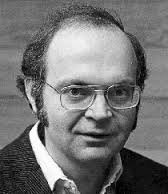
\includegraphics[width=0.15\textwidth]{figuras/donald.jpeg}
    \caption{Donald Knuth}
    \label{fig:tipografia}
\end{figure}
\end{frame}

\begin{frame}{\LaTeX{}}
    \begin{itemize}
        \item Criado por Leslie Lamport, é um conjunto de macros para o \TeX{}, facilitando a utilização de seu sistema tipográfico.
        \item Criado com a ideia de que o autor não deveria se preocupar com a formatação do texto, mas apenas em sua estrutura.
    \end{itemize}
    \begin{figure}[htbp]
    \centering
    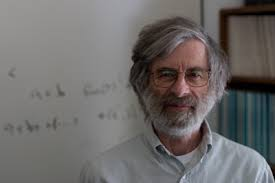
\includegraphics[width=0.25\textwidth]{figuras/leslie.jpeg}
    \caption{Leslie Lamport}
    \label{fig:leslie}
\end{figure}
\end{frame}

\begin{frame}
\begin{figure}[htbp]
    \centering
        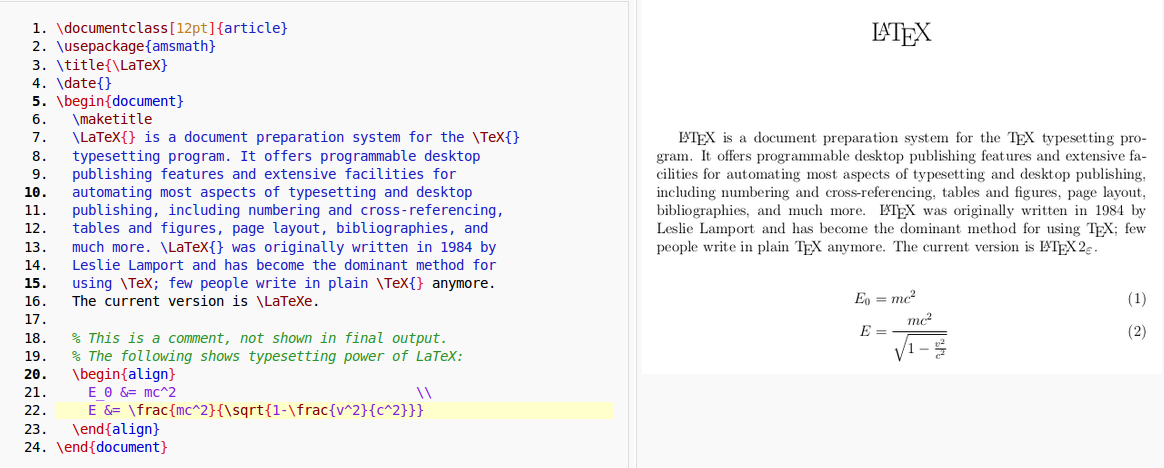
\includegraphics[width=1\textwidth]{figuras/output.png}
    \caption{\url{http://en.wikipedia.org/wiki/LaTeX}}
    \label{fig:output}
\end{figure}
\end{frame}

\section{Vantagens e Desvantagens}
\subsection{Vantagens}
\begin{frame}{Vantagens}
\begin{columns}[T]
    \begin{column}[T]{5cm}
        \begin{itemize}
            \item Software Livre;
            \item Alta qualidade tipográfica;
            \item Formatação automática dos textos;
            \item Totalmente customizável;
            \item Facilita a escrita de documentos com expressões matemáticas.
        \end{itemize}
    \end{column}

    \begin{column}[T]{5cm}
        \centering
        
\includegraphics[height=5cm]{figuras/135.png}
        %http://www.somethingofthatilk.com/index.php?id=135
    \end{column}
\end{columns}
\end{frame}

\subsection{Desvantagens}

\begin{frame}{Desvantagens}
\begin{itemize}
    \item Embora a utilização de estilos prontos de documento seja fácil, a criação de novos modelos leva muito tempo;
    \item É muito difícil escrever documentos fora de um padrão ou template;
    \item A aprendizagem é mais difícil que em editores de texto comuns.
\end{itemize}
\end{frame}

\section{Links Importantes}
\subsection{}
\begin{frame}{Fontes Importantes}
  \begin{thebibliography}{10}
  \beamertemplatearticlebibitems
  \bibitem{wiki}
    http://en.wikibooks.org/wiki/LaTeX
    \newblock \href{http://en.wikibooks.org/wiki/LaTeX}{\beamergotobutton{Link}}
    \bibitem{ctan}
    http://ctan.org/
    \newblock \href{http://ctan.org/}{\beamergotobutton{Link}}
    \bibitem{stack}
    http://tex.stackexchange.com/
    \newblock \href{http://tex.stackexchange.com/}{\beamergotobutton{Link}}
  \end{thebibliography}
\end{frame}

% \end{document}
\section{Configuração de ambiente} % (fold)
\label{sec:configura_o_de_ambiente}

\subsection{Sistemas base Unix} % (fold)
\label{sub:sistemas_base_unix}

\begin{frame}[fragile]
	\frametitle{Unix}

	Para sistemas Unix, os ambientes podem ser instalados diretamente via terminal, com o respectivo comando:

	\begin{description}
		\item [Fedora] {\code \# dnf install texlive-* texmaker ibus-qt}
		\item [Ubuntu] {\code \# apt install texlive-full texmaker ibus-qt}
		\item [Mac-OS] {\code \# brew install texlive-full texmaker ibus-qt}
	\end{description}

\end{frame}

\subsection{Sistemas base Windows} % (fold)
\begin{frame}[fragile]
	\frametitle{Windows}

	Para sistemas {\it Windows}, os executáveis podem ser localizados nos seguintes {\it links}:

	\begin{description}
		\item [MiKTeX] \href{http://ctan.sharelatex.com/tex-archive/systems/win32/miktex/}{\beamergotobutton{Link} }
		\item [TexMaker] \href{http://www.xm1math.net/texmaker/download.html#windows}{\beamergotobutton{Link} }
	\end{description}

\end{frame}


\section{Hello World}

\subsection*{Modelo de artigo básico}
\begin{frame}{Meu primeiro documento}
\begin{CenteredBox}
	\lstinputlisting{intro/carta.tex}
\end{CenteredBox}
\end{frame}

\subsection*{Modelo de artigo básico - Com título}
\begin{frame}{Minhas informações}
\begin{CenteredBox}
	\lstinputlisting[linewidth=6cm]{intro/carta1.tex}
\end{CenteredBox}
\end{frame}

\subsection*{Modelo de artigo básico - IEEE}
\begin{frame}{IEEE}
\begin{CenteredBox}
	\lstinputlisting[linewidth=6cm,basicstyle=\tiny\ttfamily]{intro/carta2.tex}
\end{CenteredBox}
\end{frame}

\subsection*{Sessões} % (fold)
\label{sub:sess_es}
\begin{frame}{Um trabalho profundo}
\begin{CenteredBox}
	\lstinputlisting[linewidth=6cm,basicstyle=\tiny\ttfamily]{intro/carta3.tex}
\end{CenteredBox}
\end{frame}
% subsection sess_es (end)

\begin{frame}
	\begin{table}[h]
	\caption{Tabela de níveis}
	\begin{center}
	\resizebox{\columnwidth}{!}{%
	\begin{tabular}{|c|c|p{5cm}|}
		\hline
		\textbf{Comando} & \textbf{Nível} & \textbf{Detalhes} \\ \hline
		\textbackslash part\{"part"\} & -1 & Não existem em cartas \\ \hline
		\textbackslash chapter\{"chapter"\} & 0 & Apenas em livros e relatórios \\ \hline
		\textbackslash section\{"section"\} & 1 & Não existem em cartas \\ \hline
		\textbackslash subsection\{"subsection"\} & 2 & Não existem em cartas \\ \hline
		\textbackslash subsubsection\{"subsubsection"\} & 3 & Não existem em cartas \\ \hline
		\textbackslash paragraph\{"paragraph"\} & 4 & Não existem em cartas \\ \hline
		\textbackslash subparagraph\{"subparagraph"\} & 5 & Não existem em cartas \\ \hline
	\end{tabular}
	}
	\end{center}
	\label{}
	\end{table}
\end{frame}

\section{Formatação básica} % (fold)

\subsection*{Caracteres Especiais} % (fold)
\label{sub:caracteres_especiais}

% subsection caracteres_especiais (end)
\label{sub:formata_o_b_sica}
\begin{frame}{Caracteres Especiais}
	\begin{description}[maiortextodomundoqueconsigoes]
		\item [{\code \%}]    Comenta linha
		% \item [{\code \textbackslash \%}]    Escreve \%
	\end{description}
\end{frame}

\begin{frame}{Caracteres Especiais}
	\begin{description}[maiortextodomundoqueconsigoes]
		\item [{\code \%}]    Comenta linha
		\item [{\code \textbackslash \%}]    Escreve \%
	\end{description}
\end{frame}

\begin{frame}{Caracteres Especiais}
	\begin{description}[maiortextodomundoqueconsigoes]
		\item [{\code \%}]    Comenta linha
		\item [{\code \textbackslash \%}]    Escreve \%
		\item [{\code \textbackslash \$}]    Escreve \$
		% \item [{\code \textbackslash \{ \}]    Escreve \{ \}
		% \item [{\code >}]    Escreve >
	\end{description}
\end{frame}


\begin{frame}{Caracteres Especiais}
	\begin{description}[maiortextodomundoqueconsigoes]
		\item [{\code \%}]    Comenta linha
		\item [{\code \textbackslash \%}]    Escreve \%
		\item [{\code \textbackslash \$}]    Escreve \$
		\item [{\code \textbackslash \_}]    Escreve \_
		% \item [{\code ><}]    Escreve ><
	\end{description}
\end{frame}

\begin{frame}{Caracteres Especiais}
	\begin{description}[maiortextodomundoqueconsigoes]
		\item [{\code \%}]    Comenta linha
		\item [{\code \textbackslash \%}]    Escreve \%
		\item [{\code \textbackslash \$}]    Escreve \$
		\item [{\code \textbackslash \_}]    Escreve \_
		\item [{\code \textbackslash \#}]    Escreve \#
	\end{description}
\end{frame}

\begin{frame}{Caracteres Especiais}
	\begin{description}[maiortextodomundoqueconsigoes]
		\item [{\code \%}]    Comenta linha
		\item [{\code \textbackslash \%}]    Escreve \%
		\item [{\code \textbackslash \$}]    Escreve \$
		\item [{\code \textbackslash \_}]    Escreve \_
		\item [{\code \textbackslash \#}]    Escreve \#
		\item [{\code \textbackslash \{ \}}]    Escreve \{ \}
	\end{description}
\end{frame}

\begin{frame}{Caracteres Especiais}
	\begin{description}[maiortextodomundoqueconsigoes]
		\item [{\code \%}]    Comenta linha
		\item [{\code \textbackslash \%}]    Escreve \%
		\item [{\code \textbackslash \$}]    Escreve \$
		\item [{\code \textbackslash \_}]    Escreve \_
		\item [{\code \textbackslash \#}]    Escreve \#
		\item [{\code \textbackslash \{ \}}]    Escreve \{ \}
		\item [{\code ><}]    Escreve ><
	\end{description}
\end{frame}
% section formata_o_b_sica (end)

\subsection*{Estilos} % (fold)
\label{sub:tamanhos}
% texttt
\begin{frame}{Estilos}
	\begin{description}[maiortextodomundoqueconsigoes]
		\item [{\code \textbackslash textbf\{negrito\}}]    Escreve \textbf{negrito}
		\item [{\code \textbackslash textit\{itálico\}}]    Escreve \textit{itálico}
	\end{description}
\end{frame}

\begin{frame}{Estilos}
	\begin{description}[maiortextodomundoqueconsigoes]
		\item [{\code \textbackslash textbf\{negrito\}}]    Escreve \textbf{negrito}
		\item [{\code \textbackslash textit\{itálico\}}]    Escreve \textit{itálico}
		\item [{\code \textbackslash texttt\{source\}}]    Escreve \texttt{source}
	\end{description}
\end{frame}

\begin{frame}{Estilos}
	\begin{description}[maiortextodomundoqueconsigoes]
		\item [{\code \textbackslash textbf\{negrito\}}]    Escreve \textbf{negrito}
		\item [{\code \textbackslash textit\{itálico\}}]    Escreve \textit{itálico}
		\item [{\code \textbackslash texttt\{source\}}]    Escreve \texttt{source}
		\item [{\code \textbackslash uppercase\{caixa\}}]    Escreve \uppercase{caixa}
		\item [{\code \textbackslash lowercase\{CAIXA\}}]    Escreve \lowercase{CAIXA}
	\end{description}
\end{frame}


\subsection*{Tamanhos} % (fold)
\label{sub:tamanhos}

\begin{frame}{Tamanhos}
	\begin{description}[maiortextodomundoqueconsigoescr]
		\item [\code \{\textbackslash tiny Excreve texto\}] 	{\tiny Escreve texto}
		\item [\code \{\textbackslash scriptsize Excreve texto\}] 	{\scriptsize Escreve texto}
		\item [\code \{\textbackslash footnotesize Excreve texto\}] 	{\footnotesize Escreve  texto}
		\item [\code \{\textbackslash small Excreve texto\}] 	{\small Escreve  texto}
		\item [\code \{\textbackslash normalsize Excreve texto\}] 	{\normalsize Escreve texto}
		\item [\code \{\textbackslash large Excreve texto\}] 	{\large Escreve  texto}
		\item [\code \{\textbackslash Large Excreve texto\}] 	{\Large Escreve  texto}
		\item [\code \{\textbackslash LARGE Excreve texto\}] 	{\LARGE Escreve  texto}
		\item [\code \{\textbackslash huge Excreve texto\}] 	{\huge Escreve  texto}
		\item [\code \{\textbackslash Huge Excreve texto\}] 	{\Huge Escreve  texto}
	\end{description}
\end{frame}


\section{Ambientes}
\begin{frame}[fragile]

Para compor textos com algum propósito especial, o \LaTeX~define
muitos tipos de ambientes para todas as classes de {\it designs}.
Em geral, um ambiente é iniciado com o comando {\code\textbackslash begin\{...\}} e encerrado com
um {\code\textbackslash end\{...\}} Tudo que está entre esses dois comandos é afetado pelo
ambiente.

\vspace{0.5cm}
\begin{center}
\begin{verbatim}
    \begin{AMBIENTE}
        ...
    \end{AMBIENTE}
\end{verbatim}
\end{center}

\end{frame}

\subsection*{Exemplos de Ambientes: Posicionamento de texto} % (fold)

\begin{frame}[fragile]
O ambiente {\bf center} permite que um texto seja centralizado na página;
{\bf flushleft} ajusta o texto à esquerda da página e {\bf ushright} coloca o texto
direita da pàgina. Um exemplo de aplicação são os comandos:

\vspace{0.5cm}
\begin{CenteredBox}
\begin{lstlisting}
\begin{center}
    Este texto ficará centralizado.
\end{center}

\begin{flushleft}
    Este texto ficará à esquerda.
\end{flushleft}

\begin{flushright}
    Este texto ficará à direita.
\end{flushright}
\end{lstlisting}
\end{CenteredBox}

\end{frame}


\begin{frame}
\begin{block}{Resultado dos comandos anteriores}
\end{block}

\begin{center}
Este texto ficará centralizado.
\end{center}

\begin{flushleft}
Este texto ficará à esquerda.
\end{flushleft}

\begin{flushright}
Este texto ficará à direita.
\end{flushright}
\end{frame}

\subsection*{Exemplos de Ambientes: Listas} % (fold)

\subsubsection*{Itemize} % (fold)
\label{ssub:itemize}

% subsubsection itemize (end)
\begin{frame}[fragile]
O \LaTeX~fornece três ambientes para a criação de listas ({\bf itemize, enumerate e description})

% Exemplo de aplicação {\bf itemize:}

\begin{columns}
\column[t]{6cm}
\begin{verbatim}
    \begin{itemize}
        \item itemize
        \item enumerate
        \item description
    \end{itemize}
\end{verbatim}
\begin{itemize}
    \item itemize
    \item enumerate
    \item description
\end{itemize}
\column[t]{6cm}
\begin{verbatim}
    \begin{enumerate}
        \item itemize
        \item enumerate
        \item description
    \end{enumerate}
\end{verbatim}
\begin{enumerate}
\item itemize
\item enumerate
\item description
\end{enumerate}

\end{columns}
\end{frame}


\subsubsection*{enumerate e description} % (fold)
\begin{frame}[fragile]
No ambiente {\bf description} os itens citados não são numerados, 
mas se utilizar um número ou uma letra entre colchetes, este será visualizado em evidenciado.

\begin{columns}
\column[t]{6cm}
\begin{verbatim}
    \begin{description}
        \item[a)] itemize
        \item[b)] enumerate
        \item[c)] description
    \end{description}
\end{verbatim}
\column[t]{6cm}
\begin{description}
\item[a)] itemize
\item[b)] enumerate
\item[c)] description
\end{description}
\end{columns}
\end{frame}


\subsection*{Exemplos de Ambientes: Matemáticos} % (fold)

\begin{frame}[fragile]
    Um dos ambientes matemáticos mais comuns é o {\code equation}.

\vspace{0.5cm}
\begin{CenteredBox}
\begin{lstlisting}
    \begin{equation}\label{eq1}
        \int_0^{15} x~dx
    \end{equation}
\end{lstlisting}
\vspace{0.5cm}
\end{CenteredBox}
    \begin{equation}\label{eq1}
        \int_0^{15} x~dx
    \end{equation}
\end{frame}

\begin{frame}[fragile]
    Para uma sequencia de equações, é possível usar o {\code eqnarray}.

\vspace{0.5cm}
\begin{CenteredBox}
\begin{lstlisting}
    \begin{eqnarray}\label{eq2}
        3x+y=2\\
        y=2-3x \nonumber \\
        y=2-3.(1)
    \end{eqnarray}\end{lstlisting}
\end{CenteredBox}

    \begin{eqnarray}\label{eq2}
        3x+y=2\\
        y=2-3x \nonumber \\
        y=2-3.(1)
    \end{eqnarray}
\end{frame}

\begin{frame}[fragile]
    Para uma sequencia de equações \textbf{alinhadas}, é possível usar o {\code align}.

\vspace{0.5cm}
\begin{CenteredBox}
\begin{lstlisting}
    \begin{align}\label{eq3}
        2x - 5y &=  8 \\ 
        3x + 9y &=  -12 - 25x + z
    \end{align}
\end{lstlisting}
\end{CenteredBox}

    \begin{align}\label{eq3}
        2x - 5y &=  8 \\ 
        3x + 9y &=  -12 - 25x + z
    \end{align}
\hrulefill\\

\vspace{0.5cm}
\begin{CenteredBox}
\begin{lstlisting}[linewidth=7.5cm]
\begin{align*}\label{eq4}
    w &=z              &  a&=b+c\\
    3w&=\frac{1}{2}z   &  a&=b\\
\end{align*}
\end{lstlisting}
\end{CenteredBox}

    % \begin{align*}\label{eq4}
    %     w &=z              &  a&=b+c\\
    %     3w&=\frac{1}{2}z   &  a&=b
    % \end{align*}

\end{frame}


\begin{frame}[fragile]
    Mas e quando queremos uma única equação com múltiplas linhas? Então usamos o {\code equation} com o {\code split}.

\vspace{0.5cm}
\begin{CenteredBox}
\begin{lstlisting}
  \begin{equation} \label{eq5}
    \begin{split}
        A & = \frac{\pi r^2}{2} \\
         & = \frac{1}{2} \pi r^2
    \end{split}
  \end{equation}
\end{lstlisting}
\end{CenteredBox}    

\begin{equation} \label{eq5}
\begin{split}
    A & = \frac{\pi r^2}{2} \\
     & = \frac{1}{2} \pi r^2
\end{split}
\end{equation}


\end{frame}

\begin{frame}[fragile]
    Todavia, quando é de interesse escrever uma equação simples em meio a um longo texto, é mais simples fazer de uso do ambiente matemático com o uso do caractere \$. 
\vspace{0.3cm}
\begin{center}
\begin{verbatim}
Texto $\oiintclockwise F(\alpha(t)),\alpha’(t)dt$ texto 
    muito longo.
  $$\lim_{h \to 0} \dfrac{f(a+h)-f(a)}{h} =: f’(a)$$
\end{verbatim}
\hrulefill\\
\vspace{0.3cm}
    Texto $\oiintclockwise F(\alpha(t)),\alpha’(t)dt$ texto  muito longo\footnote{Incluir o pacote \textit{pxfonts} para $\oiintclockwise$ funcionar.}.
\vspace{0.25cm}
    $$\lim_{h \to 0} \dfrac{f(a+h)-f(a)}{h} =: f’(a)$$
\end{center}

\end{frame}
\section{Referenciação entre labels em \LaTeX}
\begin{frame}[fragile]
\begin{block}{}
\begin{itemize}
 \item Em \LaTeX você pode facilmente referenciar quase tudo que é enumerado (sections, figures, formulas), e o \LaTeX irá  tratar o que for necessário para essas referências, atualizando sempe que houver modificações.
\end{itemize}
\end{block}
\end{frame}

\begin{frame}[fragile]
\begin{description}[maiortextodomundoqueconsigoes]
		\item [{\code \textbackslash label\{marker\}}]	Marca um objeto para futura referência
		\item [{\code \textbackslash ref\{marker\}}]    Referencia um objeto marcado
		\item [{\code \textbackslash pageref\{marker\}}]    Imprime o numero da página do objeto marcado
		\item [{\code \textbackslash nameref\{marker\}}]    Imprime o que estiver no caption do objeto marcado
	\end{description}
\end{frame}

\subsection*{Exemplo de referência de uma section}

\begin{frame}[fragile]

Exemplo de referência de uma section:

\lstinputlisting[linewidth=10cm]{citacoes/sectionExamples.tex}

\end{frame}

\begin{frame}[fragile]

Output do código anterior:

\begin{figure}[p]
   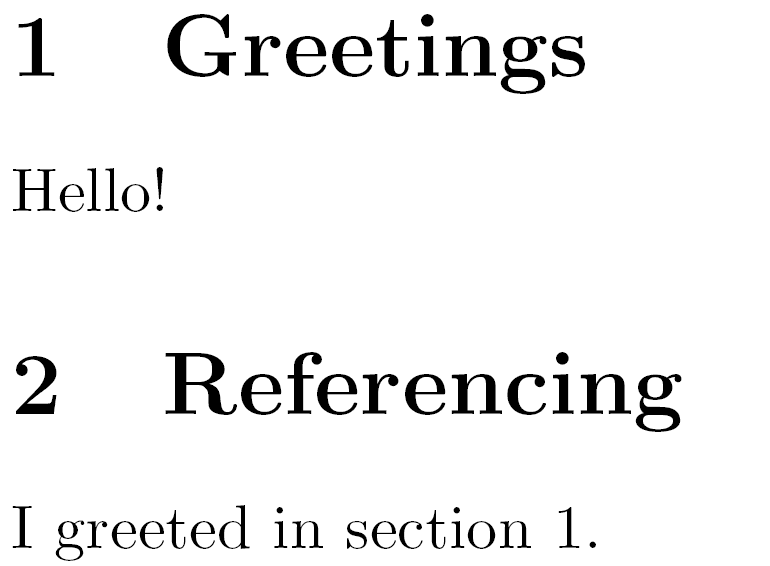
\includegraphics[scale=0.5]{figuras/sectionExample.png}
\end{figure}

\end{frame}
\section{Figuras}

\begin{frame}{Figuras no \LaTeX{}}
\begin{block}{}
\begin{itemize}
 \item O \LaTeX{} disponibiliza as facilidades básicas para trabalhar com imagens, que é um ambiente \textit{float}.
\item Um bom conjunto de comandos para essas inclusões está disponível no pacote graphicx criado por D. P. Carlisle. Esse pacote faz parte de uma família inteira de pacotes chamado de graphics bundle.
\end{itemize}
\end{block}
\end{frame}

\begin{frame}

\lstinputlisting[linewidth=8cm]{imagens/fig.tex}
Referência usando Figura \ref{fig:exemplo}

\begin{figure}[htbp!]
	\centering
	
\includegraphics[scale=0.1]{figuras/135.png}
	\caption{Nome da figura}
	\label{fig:exemplo}
\end{figure}

\end{frame}

\begin{frame}{Melhorando...}
\lstinputlisting[linewidth=8cm]{imagens/amais.tex}
\end{frame}














\section[Inclusão de códigos externos em \LaTeX]{Inclusão de códigos externos em \LaTeX~(listings)}

\begin{frame}[fragile]
\begin{block}{}
Para incluir códigos externos em seu documento \LaTeX~usamos o pacote {\it listings}. Com ele podemos:
\begin{itemize}
 \item Adicionar texto não formatado (similar ao verbatim) mas com foco em código fonte.
 \item Com ele há a possibilidade de indicar a linguagem sendo mostrada, e dependendo a formatação e apresentação muda.
 \item É possível incluir somente determinadas linhas do código fonte.
\end{itemize}
\end{block}
\end{frame}


\begin{frame}[fragile]

Para incluir código fonte sem arquivo externo basta usar o comando: 

\begin{verbatim}
\begin{lstlisting} 
    Put your code here. 
\end{lstlisting}
\end{verbatim}


\end{frame}


\begin{frame}[fragile]

Para incluir código fonte com um arquivo externo basta usar o comando: 

\begin{verbatim}
 
\lstinputlisting{source_filename.py}

\end{verbatim}


\end{frame}

\begin{frame}[fragile]

Para incluir código fonte com um arquivo externo, definir a linguagem e escolher as linhas que serão mostradas basta usar o comando: 

\begin{verbatim} 
\lstinputlisting[language=Python, 
firstline=37, lastline=45]{source_filename.py}

\end{verbatim}

Isso possibilita manter estável um \LaTeX~que gerará um documento que dependa de um código que vai mudar constantemente. Dessa forma mesmo que o código mude, o \LaTeX~permanece o mesmo e gera o documento desejado atualizado.


\end{frame}


%\begin{frame}[fragile]
%
%Para incluir código fonte com um arquivo externo basta usar o comando: 
%
%\begin{description}[maiortextodomundoqueconsigoea]
%\item [\textbackslash lstinputlisting\{source_filename.py\}]
%\end{description}
%
%\end{frame}
\section{Modelos em \LaTeX}

\begin{frame}
    Uma das facilidades do \LaTeX é  permitir que vários arquivos textos seja incluídos/importados no documento final, permitindo que um mesmo documento seja composto por vários arquivos texto.\\
    Para fazer uma inclusão de um arquivo externo, basta inserir uma das seguintes linhas:

\vspace{1cm}
\begin{center}
    {\code \textbackslash input {pasta/arquivo}}\\
    {\code \textbackslash input\{pasta/arquivo2\}}
\end{center}

\end{frame}


\begin{frame}
\subsection*{Modelos padronizados em \LaTeX} % (fold)

Na produção científica é comum a publicação de trabalhos em modelos já  prontos em \LaTeX~que já formatem automaticamente todo o texto de acordo com um padrão pré-determinado, esse modelos são amplamente utilizados em trabalhos como TCC, tese, dissertação e publicação de artigos em revistas. Alguns exemplos de podem ser encontrados no site:

\begin{center}
\url{https://www.sharelatex.com/templates/journals}
\end{center}
\end{frame}


\begin{frame}
O {\it template} utilizado exemplo será o do {\it journal Procedia Computer Science} da editora \textbf{Elsevier}.

Execute o arquivo {\code ecrc-template.tex} presente na pasta {\code\textbackslash Curso\_LaTeX\textbackslash Exemplos\textbackslash Artigo}.
\begin{figure}
\begin{center}
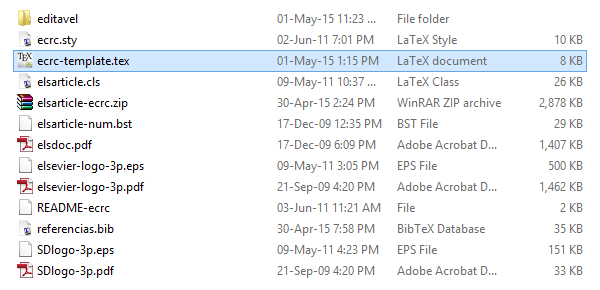
\includegraphics[scale=0.5]{figuras/figelsiever}
\caption{Template \textit{Procedia Computer Science}}
\end{center}
\end{figure}
\end{frame}

\begin{frame}[fragile]
Na linha 130 do arquivo .tex aberto inclua o comando:
\begin{verbatim}
\documentclass{beamer}

\mode<presentation> {

% The Beamer class comes with a number of default slide themes
% which change the colors and layouts of slides. Below this is a list
% of all the themes, uncomment each in turn to see what they look like.

%\usetheme{default}
%\usetheme{AnnArbor}
\usetheme{Antibes}
%\usetheme{Bergen}
%\usetheme{Berkeley}
%\usetheme{Berlin}
%\usetheme{Boadilla}                
%\usetheme{CambridgeUS} %kkkkkkkkkkkk
%\usetheme{Copenhagen}
%\usetheme{Darmstadt}  % 22222222222222
%\usetheme{Dresden}
%\usetheme{Frankfurt}
%\usetheme{Goettingen} 
%\usetheme{Hannover} %llllllllllllll
%\usetheme{Ilmenau}
%\usetheme{JuanLesPins}
%\usetheme{Luebeck}
%\usetheme{Madrid} %3333333333333333333
%\usetheme{Malmoe}
%\usetheme{Marburg}
%\usetheme{Montpellier} %2222222
%\usetheme{PaloAlto}
%\usetheme{Pittsburgh}
%\usetheme{Rochester}
%\usetheme{Singapore}
%\usetheme{Szeged} % 0000000000000000
% \usetheme{Warsaw}

% As well as themes, the Beamer class has a number of color themes
% for any slide theme. Uncomment each of these in turn to see how it
% changes the colors of your current slide theme.

%\usecolortheme{albatross}
%\usecolortheme{beaver} % 0000000000
%\usecolortheme{beetle}
%\usecolortheme{crane}
\usecolortheme{dolphin} % 0000000
%\usecolortheme{dove}   %%%%%%%%%%
%\usecolortheme{fly}
%\usecolortheme{lily}
%\usecolortheme{orchid} %%%%%%%%%%%
%\usecolortheme{rose}
%\usecolortheme{seagull}
%\usecolortheme{seahorse}
%\usecolortheme{whale}
%\usecolortheme{wolverine}

%\setbeamertemplate{footline} % To remove the footer line in all slides uncomment this line
%\setbeamertemplate{footline}[page number] % To replace the footer line in all slides with a simple slide count uncomment this line

%\setbeamertemplate{navigation symbols}{} % To remove the navigation symbols from the bottom of all slides uncomment this line
}

\usepackage{graphicx} % Allows including images
\usepackage{booktabs} % Allows the use of \toprule, \midrule and \bottomrule in tables
\usepackage[brazil]{babel}
\usepackage[T1]{fontenc}	
\usepackage[utf8]{inputenc}	
\usepackage{verbatim}
\usepackage{xcolor,lipsum}
\usepackage{listings,showexpl}
\usepackage{amsmath}
\usepackage{fancybox}
\usepackage{verbatim}
\usepackage{graphicx}
\usepackage{url}
\usepackage{multicol}
\usepackage{parcolumns}
\usepackage{pxfonts}
\usepackage{transparent}
\usepackage[font=footnotesize,labelformat=empty,
            justification=raggedright,
%            singlelinecheck=false
  ]{caption}

\pdfcompresslevel=9
\pgfdeclareimage[width=2.5cm]{logo}{logo}
\logo{\transparent{0.2}\pgfuseimage{logo}}


%--------------------------------------------
%Definições para código com fundo listrado
\newcommand\realnumberstyle[1]{#1}
\makeatletter
\newcommand{\zebra}[3]{%
    {\realnumberstyle{#3}}%
    \begingroup
    \lst@basicstyle
    \ifodd\value{lstnumber}%
        \color{#1}\pgfsetfillopacity{0.9}%
    \else
        \color{#2}%
    \fi
        \rlap{\hspace*{\lst@numbersep}%
        \color@block{\linewidth}{\ht\strutbox}{\dp\strutbox}%
        }%
    \endgroup
}
\makeatother

\lstset{%
language=tex,           %linguagem
numbers=left,           %posição dos números
stepnumber=1,           %frequencia de aparição dos números
numbersep=5pt,
numberstyle=\zebra{black!10}{white!35},
basewidth={0.6em,0.45em},
linewidth=6cm,
fontadjust=true,
mathescape=true,
tabsize=4,
commentstyle=\color{blue},
literate={á}{{\'a}}1 {à}{{\`a}}1 {ã}{{\~a}}1 {é}{{\'e}}1 {É}{{\'E}}1 {ê}{{\^e}}1 {õ}{{\~o}}1 {í}{{\'i}}1 {ó}{{\'o}}1 {ú}{{\'u}}1 {ç}{{\c c}}1 {³}{{$^3$}}1 {¢}{{\$}}1 {Ω}{{$\Omega$}}1,
% use ¢ in local to $
breaklines=true,
showstringspaces=false,
stringstyle=\color{cyan},
basicstyle=\tiny\ttfamily}

\newcommand{\code}{\small\ttfamily}
% \defbeamertemplate{description item}{align left}{\insertdescriptionitem\hfill}
% \setbeamertemplate{description item}[align left]

\makeatletter
\newenvironment{CenteredBox}{% 
\begin{Sbox}}{% Save the content in a box
\end{Sbox}\centerline{\parbox{\wd\@Sbox}{\TheSbox}}}% And output it centered
\makeatother

 \usepackage{ragged2e}
\end{verbatim}

Essa linha deve ser inserida entes do comando

\begin{verbatim}
\begin{document}

\begin{frontmatter}
\end{verbatim}

\begin{figure}
\begin{center}
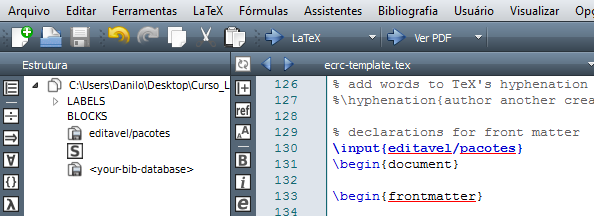
\includegraphics[scale=0.5]{figuras/fig2}
\caption{Inclusão de pacotes}
\end{center}
\end{figure}
\end{frame}



\begin{frame}[fragile]
Repita o procedimento anterior entre as linhas 160 e 180, incluindo dados conforme exposto na figura abaixo.
Compilar \textit{F6}  e visualizar o resultado \textit{F7}.
\begin{figure}
\begin{center}
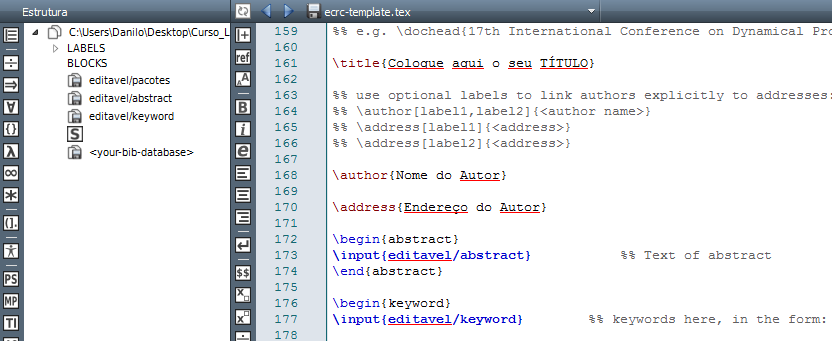
\includegraphics[scale=.5]{figuras/fig3}
\caption{Inclusão de pacotes}
\end{center}
\end{figure}
\end{frame}


\begin{frame}[fragile]
\begin{figure}
\begin{center}
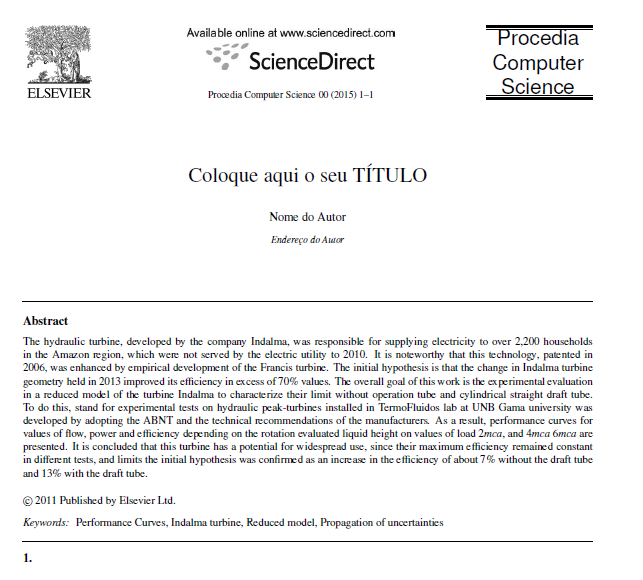
\includegraphics[scale=.4]{figuras/fig4}
\caption{Início do artigo}
\end{center}
\end{figure}
\end{frame}



\begin{frame}[fragile]
Compilar \textit{F6}, gerar referencia bibliográfica \textit{F11},  Compilar \textit{F6} e visualizar o resultado \textit{F7}.
\begin{figure}
\begin{center}
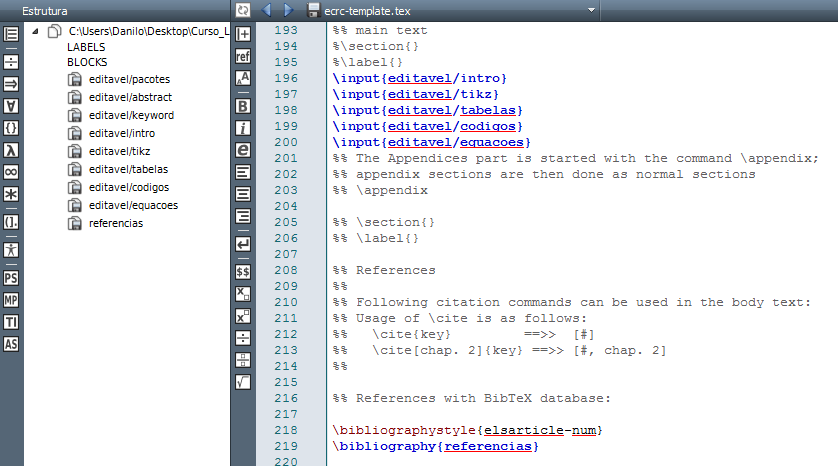
\includegraphics[scale=.5]{figuras/fig5}
\caption{Finalizando o Artigo}
\end{center}
\end{figure}
\end{frame}



\begin{frame}
No último exemplo as imagens são gráficos de forma programática, ou seja,
não foi necessário gerar um figura em um editor externo ao \LaTeX.
A criação de gráficos de forma programática gera imagens VETORIAIS, exemplos podem ser encontrados em:

\vspace*{0.5cm}
\begin{center}
\textit{http://www.texample.net/tikz/}
\end{center}
\vspace*{0.5cm}

Outros exemplos estão disponíveis na pasta "$\backslash Curso\_ LaTeX \backslash Exemplos$". 
Os exemplos nas pastas "$DocHell$" e "$Fisica\_moderna$" devem ser executados no arquivo "$main.tex$"
\end{frame}



\section{Tabelas} % (fold)
\label{sec:tabelas}

\subsection*{Código} % (fold)
\label{sub:c_digo}


% % subsection c_digo (end)
% % section tabelas (end)

\begin{frame}

\lstinputlisting[linewidth=10cm]{tables/table.tex}
\begin{table}[h]
	\caption{Tabela de Exemplo}
	\begin{tabular}{l|c|l||r||p{3cm}}
		0 & 1 & Texto & 3 & Texto muito longo para célula\\
		4 & Texto & 7 & $\int_0^1 2x dx$ & 9 \\ \hline
		&  & $\partial$ &  &
	\end{tabular}
	\label{tab:exemplo}
\end{table}

\end{frame}
\section{Referências Bibliográficas}

\begin{frame}{Referências Bibliográficas}
\begin{itemize}
 \item A forma mais simples de se referenciardentro de um texto é usando o ambiente {\ttfamily thebibliography}.
\item Entretanto, o Bib\TeX{} é uma ferramenta que oferece muito mais flexibilidade na formatação dos textos.
\end{itemize}
\end{frame}

\begin{frame}{Configurando o documento}
\lstinputlisting{citacoes/biblio.tex}
\end{frame}

\subsection{Coletando citações}

\begin{frame}{Use o \href{http://scholar.google.com.br}{Google Acadêmico}}
	
\begin{figure}[htbp!]
	\centering
	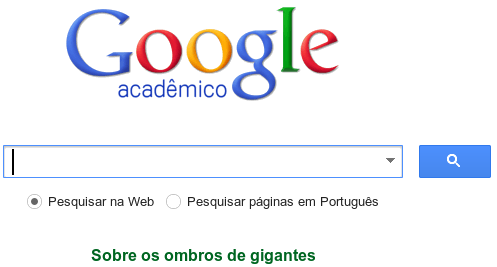
\includegraphics[width=0.6\textwidth]{figuras/google1.png}
	\caption{ }
\end{figure}
\end{frame}

\begin{frame}{Coletando citações}
	
\begin{multicols}{2}
\begin{figure}[htbp!]
	% \centering
	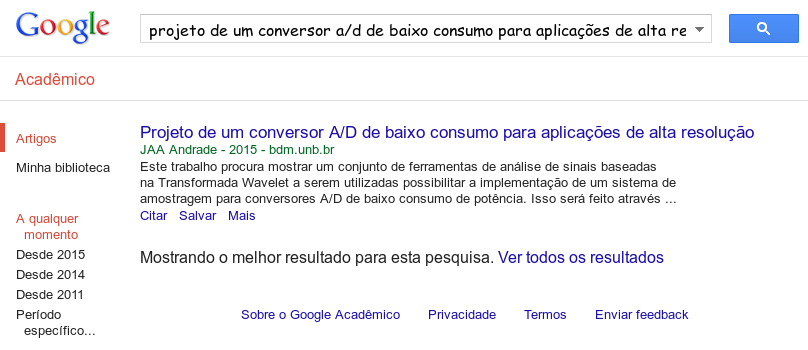
\includegraphics[width=0.6\textwidth]{figuras/google2.png}
	\caption{ }
\end{figure}
	
\begin{figure}[htbp!]
	\centering
	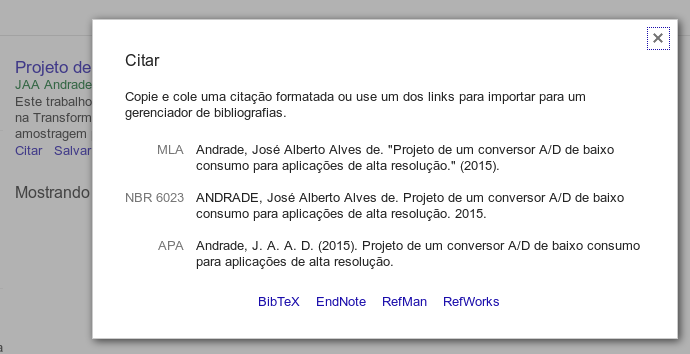
\includegraphics[width=0.4\textwidth]{figuras/google3.png}
	\caption{ }
\end{figure}
\end{multicols}
\end{frame}

\begin{frame}[fragile]{Coletando citações}

\begin{lstlisting}[linewidth=10cm]
@article{andrade2015projeto,
  title={Projeto de um conversor A/D de baixo consumo para aplica{\c{c}}{\~o}es de alta resolu{\c{c}}{\~a}o},
  author={Andrade, Jos{\'e} Alberto Alves de},
  year={2015}
}
\end{lstlisting}
	
\end{frame}
\section{Glossários} 
\begin{frame}{Declarando}
\lstinputlisting[linewidth=8cm,basicstyle=\tiny\ttfamily]{glossaries/glo}	
\end{frame}

\begin{frame}{Fazendo uso}
	
Faça uso no texto com {\ttfamily \textbackslash gls\{UC\}}, \gls{UC}.

\end{frame}

\begin{frame}
	\glossarystyle{altlisthypergroup}
	\printglossaries
\end{frame}

\section{Tikz} % (fold)
\label{sec:tikz}

\begin{frame}{O que é?}
\begin{block}{}
	\begin{itemize}
		\item Um dos melhores pacotes para {\bf produzir} gráficos \underline{vetorizados} em \LaTeX.
		\item Possui um extensa \href{http://ftp.fau.de/ctan/graphics/pgf/base/doc/pgfmanual.pdf}{documentação}.
		\item Disponibiliza diversos \href{http://www.texample.net/tikz/examples/}{exemplos} de como utilizar o pacote.
	\end{itemize}
\end{block}
\end{frame}

\subsection*{Vantagens \& Desvantagens}
\begin{frame}{Vantagens}
	\begin{multicols}{2}		
	\input tikz/gnuplot
	\input tikz/polar
	\end{multicols}
\end{frame}

% section tikz (end)
\begin{frame}{Vantagens}
	\begin{multicols}{2}		
	\input tikz/square
	\input tikz/circuitikz
	\end{multicols}
\end{frame}


\begin{frame}{Desvantagens}
	\begin{block}{}
		\begin{itemize}
			\item Péssima curva de aprendizado.
			\item Desalinhamento de  versões entre o disponibilizado nos repositórios com os apresentados nos exemplos.
			\item {\it Sujo}
		\end{itemize}
	\end{block}
\end{frame}

\subsection*{Exemplos}
\begin{frame}{Circuito}
	\lstinputlisting[linewidth=8cm,basicstyle=\tiny\ttfamily]{tikz/circuitikz.tex}
\end{frame}

\begin{frame}{GnuPlot}
	\lstinputlisting[linewidth=8cm,basicstyle=\tiny\ttfamily]{tikz/gnuplot.tex}
\end{frame}

\section*{}
\begin{frame}
\begin{center}
  \Huge\ttfamily \textbf {OBRIGADO!}
\end{center}
\end{frame}


\end{document}
